\documentclass[border=3pt,varwidth]{standalone}
\usepackage{amsmath,amssymb}
\usepackage{tikz}
\usetikzlibrary{arrows.meta,calc,decorations.markings,patterns,positioning,angles,quotes}
\tikzset{
  >=Stealth,
  every node/.style={font=\normalsize},
  wire/.style={line width=0.9pt},
  thinwire/.style={line width=0.6pt},
  fieldline/.style={line width=0.6pt,-{Stealth[length=2.2mm]}},
  axis/.style={line width=0.7pt,-{Stealth[length=2.2mm]}},
  dashedwire/.style={line width=0.9pt,dash pattern=on 3pt off 2pt},
  resistor/.style={line width=0.9pt},
  chargepos/.style={circle,draw,line width=0.8pt,minimum size=5mm,inner sep=0pt},
  dotcharge/.style={circle,fill,inner sep=0pt,minimum size=2.4pt}
}
% Draw a resistor box centered at (x,y) with width w, height h, horizontal
\newcommand{\resbox}[4]{%
  % #1=x #2=y #3=halfwidth #4=label
  \draw[resistor] (#1-#3,#2-0.18) rectangle (#1+#3,#2+0.18);
  \ifx\\#4\\\else\node[above=2pt] at (#1,#2+0.18) {#4};\fi
}
% Battery symbol: long thin line (+) then short thick line (-), centered at (x,y)
\newcommand{\battery}[2]{%
  % #1=x #2=y ; long line left=+, short line right=- by default orientation
  \draw[wire] (#1-0.09,#2-0.32) -- (#1-0.09,#2+0.32);
  \draw[line width=2.6pt] (#1+0.09,#2-0.16) -- (#1+0.09,#2+0.16);
}

\begin{document}
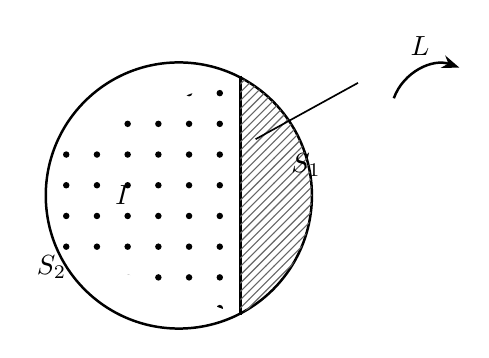
\begin{tikzpicture}[scale=1.3]
  \def\R{1.3}
  % chord endpoints splitting the circle: small wedge S1 on the right, S2 the rest
  \coordinate (P1) at (0.60,1.17);
  \coordinate (P2) at (0.60,-1.17);
  \draw[wire] (0,0) circle (\R);
  \draw[wire] (P1) -- (P2);
  % S1: hatched lens-shaped region on the right (small sliver)
  \begin{scope}
    \clip (0,0) circle (\R);
    \clip (P1) -- (P2) -- (2.6,0) -- cycle;
    \fill[pattern=north east lines, pattern color=black!60] (0,0) circle (\R);
  \end{scope}
  % S2: dotted region (current out of page) on the left, majority of circle
  \begin{scope}
    \clip (0,0) circle (\R);
    \clip (P1) -- (P2) -- (-2.6,0) -- cycle;
    \foreach \x in {-1.1,-0.8,...,1.1} {
      \foreach \y in {-1.1,-0.8,...,1.1} {
        \fill (\x,\y) circle (0.9pt);
      }
    }
  \end{scope}
  \node at (-0.55,0) {$I$};
  \node[left=2pt] at (-0.95,-0.7) {$S_2$};
  \node[right=2pt] at (0.95,0.3) {$S_1$};
  % loop arrow L outside the circle, upper right, with a leader line to the wedge
  \draw[thinwire] (0.75,0.55) -- (1.75,1.1);
  \draw[wire,-{Stealth[length=2.2mm]}] (2.1,0.95) arc[start angle=160,end angle=70,radius=0.5];
  \node[above right=1pt] at (2.15,1.25) {$L$};
\end{tikzpicture}
\end{document}
